%\documentclass[a4paper]{article}
%\usepackage{beamerarticle}

\documentclass[ignorenonframetext]{beamer}
\usepackage{beamerthemesplit}
\usepackage{amssymb}

\usepackage{../fhnw-beamer}

%\mode<article>{\usepackage{fullpage}}
%\mode<presentation>{\usetheme{Berlin}}

\date{\today}
\author{rolf.schmutz@fhnw.ch}
\institute{FHNW}
\title {Netzwerke und Datenkommunikation\\NDK 02-050\\Layer-3 IP part 3\\ARP + ICMP}


\begin{document} % ===============================================================

\section{NDK 02-050: IP, Part 3}



\begin{frame}
\titlepage
\end{frame}

\begin{frame}
\frametitle{Ziele}
\begin{itemize}
	\item{Sie kennen die Adresszuweisung L3$\leftrightarrow$L2, ARP}
	\item{Sie kennen das Fehlermeldungs/Test-Protokoll ICMP und einige Anwendungen davon}
	\item{Praktische Erfahrung mit einfachen IP-inter-Netzwerken}
%\item{Sie kennen die Verwendung der RFC1918 {\em private addresses} und die dazu n\"otigen Vorkehrungen}
\end{itemize}
\end{frame}




\begin{frame}
\frametitle{Spezielle IP-Adressen}
einige Bereiche im IP-Adressraum sind f\"ur spezielle Anwendungen reserviert:
\begin{small}
\begin{center}
\begin{tabular}{|c|l|l|}
\hline 
\textbf{IP} & \textbf{Bedeutung} & \textbf{Source/Destination} \\
0.0.0.0 & unbekannte Source \tiny{(DHCP/BOOTP)} & nur Source \\
255.255.255.255 & limited Broadcast & nur Destination\tiny{, stoppt am Router} \\
127.0.0.0/8 & loopback\tiny{, Host-lokal} & beides, nur Host-intern \\
192.168.0.0/16 & {\em private} IP\tiny{, RFC1918, braucht NAT f\"ur Internet} & beides\tiny{, wird im Internet nicht geroutet} \\
172.16.0.0/12 & {\em private} IP\tiny{, RFC1918, braucht NAT f\"ur Internet} & beides\tiny{, wird im Internet nicht geroutet} \\
10.0.0.0/8 & {\em private} IP\tiny{, RFC1918, braucht NAT f\"ur Internet} & beides\tiny{, wird im Internet nicht geroutet} \\
169.254.0.0/16 & Link-Local\tiny{, automatisch IPs ohne DHCP} & beides\tiny{, wird im Internet nicht geroutet} \\
\hline
10.195.5.0/24 & Netz-Basisadresse\tiny{, alle Hostbits=0} & keine \\
10.195.5.255/24 & directed Broadcast\tiny{, alle Hostbits=1} & nur Destination \\
\hline 
\end{tabular}
\end{center}
\end{small}
\myurl{http://www.inetdaemon.com/tutorials/internet/ip/addresses/special.shtml}\\
\myurl{http://de.wikipedia.org/wiki/IP-Adresse\#Besondere_IP-Adressen}\\
\myurl{http://www.rfc-editor.org/rfc/pdfrfc/rfc1918.txt.pdf}
\end{frame}




\begin{frame}[fragile]
\frametitle{ARP: Address Resolution Protocol, 1/2}
\begin{itemize}
  \item{ARP findet zu einer gew\"unschten IP-Adresse die entsprechende MAC-Adresse: L3?$\rightarrow$L2 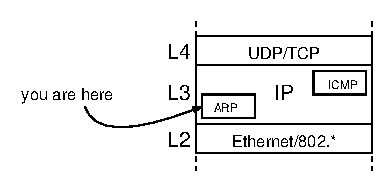
\includegraphics[height=1.5cm]{arp-layer}}
  \item{\begin{tiny}\begin{verbatim}tcpdump -l -e -nnn arp
10:33:07.377978 00:26:18:ce:27:6d > ff:ff:ff:ff:ff:ff, ethertype ARP (0x0806), length 42: 
                Request who-has 192.168.1.17 tell 192.168.1.16, length 28
10:33:07.378086 00:0d:b9:16:bf:e4 > 00:26:18:ce:27:6d, ethertype ARP (0x0806), length 60: 
                Reply 192.168.1.17 is-at 00:0d:b9:16:bf:e4, length 46
\end{verbatim}\end{tiny}}
  \item{RARP ist das ``R\"uckw\"artsprotokoll'': 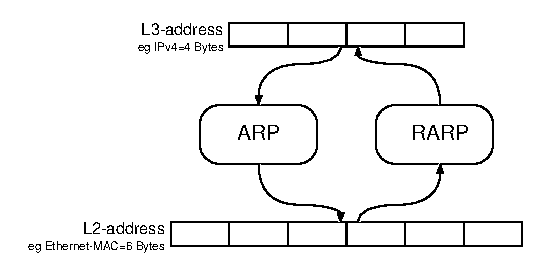
\includegraphics[height=1.5cm]{arp-opschema}}
  \item{ARP und RARP arbeiten beide mit L2/MAC-Broadcasts f\"ur die Anfragen und L2-Unicast f\"ur die Antworten\footnote{\ldots meistens. Deshalb sehen Sie mit \texttt{tcpdump} nur die ARP-Anfragen (Broadcast)}}
\end{itemize}
\end{frame}

\begin{frame}
\frametitle{ARP: Address Resolution Protocol, 2/2}
\begin{itemize}
  \item{Ablauf und Kommunikation} \vspace{0.25cm}
  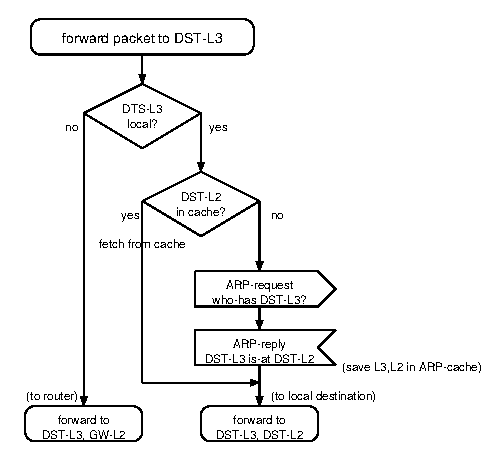
\includegraphics[width=5cm]{arp-procedure} 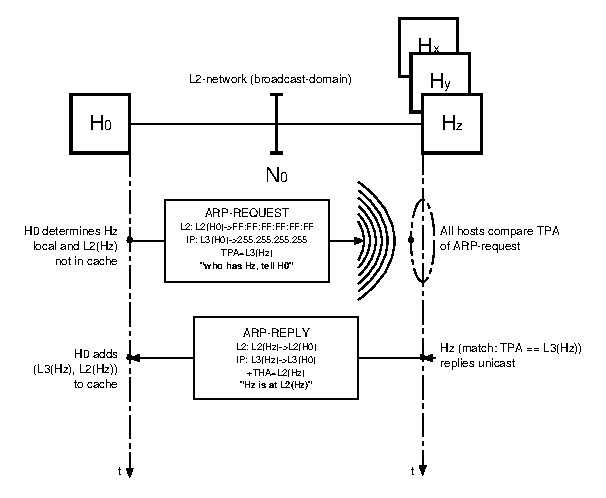
\includegraphics[width=5cm]{arp-communication}
  \item{Tools: ARP-Cache angucken, l\"oschen oder statische Eintr\"age einf\"ugen: \texttt{arp}}
\end{itemize}
\end{frame}



\begin{frame}
\frametitle{ICMP, Internet Control Message Protocol, 1/3}
IP (Layer-3) ist {\em best-effort}{}\footnote{Pakete k\"onnen verloren gehen}, d.h. es wird ein Mechanismus zur Fehlersignalisation ben\"otigt: 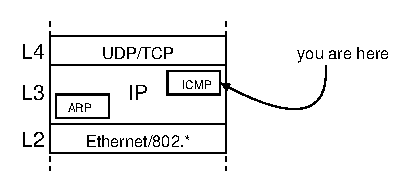
\includegraphics[height=1.5cm]{icmp-layer}
\begin{itemize}
  \item{ICMP implementiert {\em Fehlermeldungen} und {\em Statusabfragen} in TCP/IP}
  \item{Router k\"onnen durch ICMP Fehlerindikationen an das sendende Ger\"at zukommen lassen\footnote{\ldots normalerweise sind Router ``stumm'', resp. d\"urfen nicht in die Kommunikation eingreifen}}
  \item{Die Meldungen sind mit einem Code/Bedeutung markiert und enthalten den Original IP-Header des verursachenden Pakets\footnote{um dem Ger\"at die Zuweisung des Fehlers an das betroffene Programm zu erm\"oglichen (z.B. browser)}}
  \item{bei den meisten Fehlermeldungen wird das Original-Paket verworfen, der Sender muss versuchen es erneut zuzustellen oder die Fehlermeldung an die Applikation weiterzuleiten}
\end{itemize}
\end{frame}

\begin{frame}
\frametitle{ICMP, Internet Control Message Protocol, 2/3}
\begin{itemize}
	\item{Fehlermeldungen: erm\"oglicht Router und Endger\"ate die Paketquelle \"uber Fehler zu informieren (Auswahl)\\   \begin{tiny}
	    \begin{tabular}{|l|l|l|l|}
	      \hline
	      \textbf{Meldung} & \textbf{Bedeutung} & \textbf{Sender} & Verworfen \\
	      \hline
	      network unreachable & kein passender Routing-Table Eintrag & Router & Paket verworfen \\
	      host unreachable & keine Antwort auf ARP & letzter Router & Paket verworfen \\
	      port unreachable & kein Serverprozess, Listen-Socket & Zielhost & Paket verworfen \\
	      time exceeded & TTL abgelaufen\footnote{{\em Time To Live} ist ein numerisches Feld im IP-Header und wird von jedem Router dekrementiert (-1) -- bei 0 $\rightarrow$ time-exceeded} & Router & Paket verworfen \\
	      fragmentation needed & Paket zu gross & Router & Paket verworfen \\
	      redirect & an anderen Router senden\footnote{enth\"alt IP des ``besseren'' Routers $\rightarrow$ Routing-Table} & Router & Paket weitergeleitet \\
	      source-quench & Flusskontrolle, veraltet\footnote{\ldots da meistens ignoriert und zus\"atzlicher Aufwand (Status) f\"ur Router} & Router & Paket weitergeleitet \\
	      \hline
	    \end{tabular}
	  \end{tiny}
	}
	\vspace{0.25cm}
	\item{Statusabfragen: erm\"oglicht einfache Statusabfragen auf Layer-3}\\    \begin{tiny}
	    \begin{tabular}{|l|l|l|}
	      \hline
	      \textbf{Meldung} & \textbf{Bedeutung} & \textbf{Sender} \\
	      \hline
				echo-request und echo-reply & Erreichbarkeitstest\footnote{z.B. \texttt{ping}} auf Layer-3 & alle \\
				timestamp-request und -reply & Zeitstempel\footnote{enth\"alt Local-Absende-, Remote-Empfangs- und Absende-Zeitstempel. Local-Empfangszeitstempel wird bei Erhalt der -reply-Meldung eingetragen} Abfrage & alle \\
	      \hline
	    \end{tabular}
	  \end{tiny}
\end{itemize}
\end{frame}


\begin{frame}
\frametitle{ICMP, Internet Control Message Protocol, 3/3}
{\center 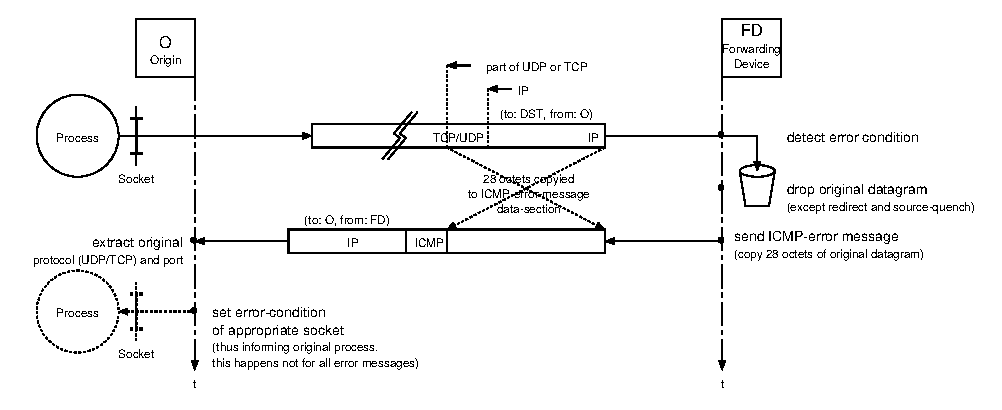
\includegraphics[height=5cm]{icmp-errormessage}} \\
{\center 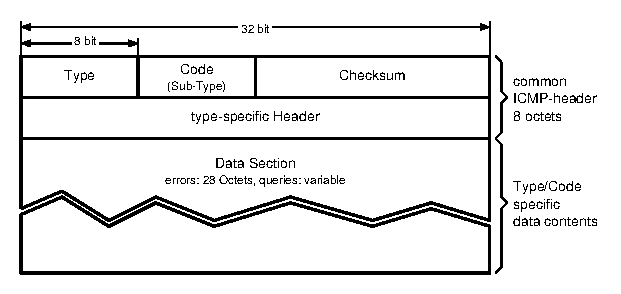
\includegraphics[height=2cm]{icmp-packetformat}}
\end{frame}

\begin{frame}[fragile]
\frametitle{ICMP Tools 1/2}
\begin{itemize}
	\item{\textbf{\texttt{ping}}: Layer-3 reachability} testen Erreichbarkeit\footnote{mit Hilfe von ICMP-echo-request Meldungen} auf Layer-3:
		\begin{tiny}
		\begin{verbatim}
rschmutz@callisto ~ $ ping -c 3 www.google.ch
PING www.l.google.com (209.85.227.99): 56 data bytes
64 bytes from 209.85.227.99: icmp_seq=0 ttl=54 time=44.935 ms
64 bytes from 209.85.227.99: icmp_seq=1 ttl=54 time=41.854 ms
64 bytes from 209.85.227.99: icmp_seq=2 ttl=54 time=58.240 ms

--- www.l.google.com ping statistics ---
3 packets transmitted, 3 packets received, 0.0% packet loss
round-trip min/avg/max/stddev = 41.854/48.343/58.240/7.110 ms
\end{verbatim}
\end{tiny}
\item{\texttt{ping}/ICMP-Echo-Request testet nur die \emph{Erreichbarkeit auf Schicht-3 ``End-zu-end System''}\footnote{d.h. IP-Adresse/Host kann erreicht werden aber keine Angaben \"uber die Verf\"ugbarkeit eines speziellen Dienstes (Mail, Web, etc) auf diesem Host}}
\item{ICMP-Echo-Request/Response wird h\"aufig auf Firewalls ``geblockt''
  \begin{itemize}
    \item{\texttt{ping} auf eine Adressen/Host ergibt keine Antwort (timeouts) \emph{aber} der HTTP-Dienst auf derselben Adresse/Host ist verf\"ugbar\footnote{z.B. \texttt{ping www.microsoft.com}$\rightarrow$nix aber \texttt{http://www.microsoft.com/} im Browser funktioniert}}
  \end{itemize}
}
\item{die Ausgabe ist normalerweise die ``Round-Trip-Time'', d.h. die total ben\"otigte Zeit Anfrage+Verarbeitung+Antwort}
\end{itemize}
\end{frame}


\begin{frame}[fragile]
\frametitle{ICMP Tools 2/2}
\begin{itemize}
	\item{\textbf{\texttt{traceroute}}: Layer-3 route path\footnote{durch erzwingen von 		ICMP-time-exceeded und ICMP-port-unreachable Meldungen}}
\begin{tiny}
		\begin{verbatim}
rschmutz@zaphod:~$ traceroute www.google.com
traceroute to www.google.com (209.85.135.103), 30 hops max, 40 byte packets
 1  static.193.65.40.188.clients.your-server.de (188.40.65.193)  0.676 ms  0.702 ms  0.723 ms
 2  hos-tr1.juniper1.rz10.hetzner.de (213.239.227.129)  0.189 ms  0.194 ms
    hos-tr4.juniper2 (213.239.227.225)  0.178 ms
 3  hos-bb1.juniper2.ffm.hetzner.de (213.239.240.226)  4.559 ms  4.576 ms  4.597 ms
 4  de-cix10.net.google.com (80.81.192.108)  5.682 ms  5.981 ms  6.331 ms
 5  209.85.255.172 (209.85.255.172)  6.098 ms
    209.85.255.170 (209.85.255.170)  16.070 ms  6.192 ms
 6  72.14.238.128 (72.14.238.128)  14.460 ms  14.001 ms
    209.85.248.248 (209.85.248.248)  11.706 ms
 7  209.85.241.187 (209.85.241.187)  13.981 ms
    209.85.241.83 (209.85.241.83)  13.886 ms  14.033 ms
 8  209.85.253.22 (209.85.253.22)  13.074 ms  13.896 ms
    72.14.239.54 (72.14.239.54)  27.321 ms
 9  mu-in-f103.1e100.net (209.85.135.103)  15.272 ms  15.526 ms  13.659 ms
\end{verbatim}
\end{tiny}
\item{\texttt{traceroute} zeigt den scheinbaren ``Pfad''\footnote{IP=Paketvermittelnd $\rightarrow$ \emph{kein} ``Pfad'', d.h. \texttt{traceroute} l\"ugt ein bisschen} -- d.h. die einzelnen Router + Distanz in ``hops'' -- zu einer Zieladresse}
\item{dazu werden TTL-begrenzte Pakete\footnote{z.B. UDP-Pakete an m\"oglichst unbenutzte Ports} ausgesendet und die ICMP-Time-Exceeded-in-Transit Meldungen der Router ausgegeben}
\item{wie auch \texttt{ping} wird \texttt{traceroute} h\"aufig ``geblockt'' und zudem sind die Angaben interpretationsbed\"urftig}
\end{itemize}
\end{frame}














\begin{frame}[fragile]
\frametitle{Tool References 1/2}
\begin{itemize}
	\item \texttt{ping} Windos:
	\begin{tiny}
	\begin{verbatim}
Syntax: ping [-t] [-a] [-n Anzahl] [-l Groesse] [-f] [-i TTL] [-v TOS]
             [-r Anzahl] [-s Anzahl] [[-j Hostliste] | [-k Hostliste]]
             [-w Zeitlimit] [-R] [-S Quelladresse] [-4] [-6] Zielname

Optionen:
    -t             Sendet fortlaufend Ping-Signale zum angegebenen Host.
                   Geben Sie STRG-UNTRBR ein, um die Statistik anzuzeigen.
                   Geben Sie STRG-C ein, um den Vorgang abzubrechen.
    -a             L�st Adressen in Hostnamen auf.
    -n Anzahl      Anzahl der zu sendenden Echoaufforderungen.
    -l Groesse     Sendet Pufferlaenge.
    -f             Setzt Flag f�r "Nicht fragmentieren" im Paket (nur IPv4).
    -i TTL         Gueltigkeitsdauer (TTL).
    -r Anzahl      Route f�r Anzahl der Abschnitte (nur IPv4).
	\end{verbatim}
	\end{tiny}
	\item \texttt{ping} UNIX (Darwin):
	\begin{tiny}
	\begin{verbatim}
usage: ping [-AaDdfnoQqRrv] [-b boundif] [-c count] [-G sweepmaxsize] [-g sweepminsize]
            [-h sweepincrsize] [-i wait] [-l preload] [-M mask | time] [-m ttl]
            [-p pattern] [-S src_addr] [-s packetsize] [-t timeout]
            [-W waittime] [-z tos] host
       ping [-AaDdfLnoQqRrv] [-c count] [-I iface] [-i wait] [-l preload]
            [-M mask | time] [-m ttl] [-p pattern] [-S src_addr]
            [-s packetsize] [-T ttl] [-t timeout] [-W waittime]
            [-z tos] mcast-group
	\end{verbatim}
	\end{tiny}
\end{itemize}
\end{frame}


\begin{frame}[fragile]
\frametitle{Tool References 2/2}
\begin{itemize}
	\item \texttt{traceroute} UNIX (Darwin):
	\begin{tiny}
	\begin{verbatim}
Usage: traceroute [-adDeFInrSvx] [-A as_server] [-f first_ttl] [-g gateway] [-i iface]
	[-M first_ttl] [-m max_ttl] [-p port] [-P proto] [-q nqueries] [-s src_addr]
	[-t tos] [-w waittime] [-z pausemsecs] host [packetlen]
	\end{verbatim}
	\end{tiny}
	\item \texttt{tracert} Windos:
	\begin{tiny}
	\begin{verbatim}
Syntax: tracert [-d] [-h Max. Abschnitte] [-j Hostliste] [-w Zeitlimit]
                [-R] [-S Quelladresse] [-4] [-6] Zielname

Optionen:
    -d                  L�st Adressen nicht in Hostnamen auf.
    -h Max. Abschnitte  Maximale Anzahl an Abschnitten bei Zielsuche
    -j Hostliste        "Loose Source Route" gemaess Hostliste (nur IPv4)
    -w Zeitlimit        Zeitlimit in Millisekunden f�r eine Antwort
	\end{verbatim}
	\end{tiny}
\end{itemize}
\end{frame}


%\begin{frame}
%\frametitle{NAT: Network Address Translation}
%\end{frame}




\begin{frame}
\frametitle{References}
\begin{itemize}
	\item{Spezielle IP Adressen: \myurl{http://www.inetdaemon.com/tutorials/internet/ip/addresses/special.shtml}}
	\item{Spezielle IP Adressen: \myurl{http://de.wikipedia.org/wiki/IP-Adresse\#Besondere_IP-Adressen}}
	\item{NAT \myurl{http://datatracker.ietf.org/doc/rfc1918/}}
	\item{private address space \myurl{http://www.rfc-editor.org/rfc/pdfrfc/rfc1918.txt.pdf}}
\end{itemize}
\end{frame}





\end{document}